\documentclass{amsart}
\usepackage{graphicx}
\graphicspath{{./}}
\usepackage{hyperref}
\usepackage{csvsimple}
\usepackage{longtable}
\usepackage{epigraph}
\title{Romantic Love and Psychological Changes Most Important For Human Evolution from Homo Australopithecus}
\author{Zulfikar Moinuddin Ahmed}
\date{\today}
\begin{document}
\maketitle

\section{Homo Austraulopithecus had Romantic Love}

Romantic Love is necessary whenever the primate brain is too big for the baby to fit past the hip girth of the female.  For then the infant has a long period of helplessness till maturity of the brain and paternal investment in raising the infant is necessary.  This is the crucial new insight I have about the origins of Human Race: that Romantic Love came before growth of the brain.  Romantic Love sparked the birth of the Human Race and it's ancestors.

\section{Centrality of Psychological Development}

Much of physical study of origins of human race is based on fossil evidence which is great work, and grueling and rewarding work of great labour.  I just received a copy of {\em The Complete World of Human Evolution} and there is a natural interest in physical features of ancestors of Homo Sapiens.  For me it is important to take a distance from the focus on fossils and consider the psychological evolution.  Romantic Love is a central issue but other social emotions and instincts are also important.  

Now Homo Austraulopithecus stood upright on two legs.  This was the marvelous discovery of Raymond Dart in the 1920s which is marvelous.  The genus Homo descended from species Austraulopithecus between 3 and 2 million years ago, while Homo Austraulopithecus itself became extinct 1.9 Mya.
  

\section{Today Murder Rates are Uniformly Below 0.08 percent across the Globe}

It is worth interpolating very roughly from 2021 to 3 Mya. We are the Human Race, Homo Sapiens, but including all the ancestor races and cousing back to Homo Australopithecus 3 Mya, we can make the parsimonious assumption that the murder rate was not wildly higher than 0.08 percent for the group of species.  This is my {\em Human Ancestral Violence Hypothesis}.  

\section{Morality of Violence Against Others In 49 Countries}

Table of $\lambda$ parameter estimates for 49 countries.

% latex table generated in R 4.0.3 by xtable 1.8-4 package
% Thu Apr 22 19:20:11 2021
\begin{longtable}{rrrr}
  \hline
 & B\_COUNTRY & lambda & rsq \\ 
  \hline
1 & 20 & -0.7006 & 0.88 \\ 
  2 & 32 & -0.4609 & 0.74 \\ 
  3 & 36 & -0.4970 & 0.76 \\ 
  4 & 50 & -0.9417 & 0.97 \\ 
  5 & 68 & -0.4814 & 0.76 \\ 
  6 & 76 & -0.3455 & 0.49 \\ 
  7 & 152 & -0.3842 & 0.79 \\ 
  8 & 156 & -0.5324 & 0.65 \\ 
  9 & 170 & -0.3923 & 0.51 \\ 
  10 & 196 & -0.4750 & 0.76 \\ 
  11 & 276 & -0.8491 & 0.85 \\ 
  12 & 218 & -0.3471 & 0.57 \\ 
  13 & 818 & -1.2017 & 0.83 \\ 
  14 & 231 & -0.3751 & 0.18 \\ 
  15 & 300 & -0.6164 & 0.66 \\ 
  16 & 320 & -0.3195 & 0.74 \\ 
  17 & 344 & -0.5007 & 0.91 \\ 
  18 & 360 & -0.5145 & 0.78 \\ 
  19 & 364 & -0.4984 & 0.72 \\ 
  20 & 368 & -0.4446 & 0.91 \\ 
  21 & 400 & -0.4870 & 0.75 \\ 
  22 & 392 & -0.6113 & 0.47 \\ 
  23 & 398 & -0.3707 & 0.72 \\ 
  24 & 417 & -0.3398 & 0.43 \\ 
  25 & 410 & -0.5752 & 0.88 \\ 
  26 & 422 & -0.5346 & 0.94 \\ 
  27 & 446 & -0.5359 & 0.93 \\ 
  28 & 484 & -0.3086 & 0.72 \\ 
  29 & 104 & -0.7837 & 0.75 \\ 
  30 & 458 & -0.2532 & 0.80 \\ 
  31 & 566 & -0.4910 & 0.69 \\ 
  32 & 558 & -0.3444 & 0.45 \\ 
  33 & 554 & -0.5083 & 0.66 \\ 
  34 & 586 & -0.3654 & 0.65 \\ 
  35 & 604 & -0.4728 & 0.81 \\ 
  36 & 608 & -0.1854 & 0.55 \\ 
  37 & 630 & -0.3658 & 0.46 \\ 
  38 & 642 & -0.4364 & 0.68 \\ 
  39 & 643 & -0.3972 & 0.87 \\ 
  40 & 688 & -0.2148 & 0.16 \\ 
  41 & 764 & -0.5786 & 0.92 \\ 
  42 & 762 & -0.6506 & 0.83 \\ 
  43 & 788 & -0.5442 & 0.87 \\ 
  44 & 792 & -0.4655 & 0.77 \\ 
  45 & 158 & -0.6305 & 0.86 \\ 
  46 & 804 & -0.5147 & 0.93 \\ 
  47 & 840 & -0.4576 & 0.79 \\ 
  48 & 704 & -0.4523 & 0.86 \\ 
  49 & 716 & -0.2702 & 0.27 \\ 
   \hline
\hline
\end{longtable}

The histogram shows a GHD.
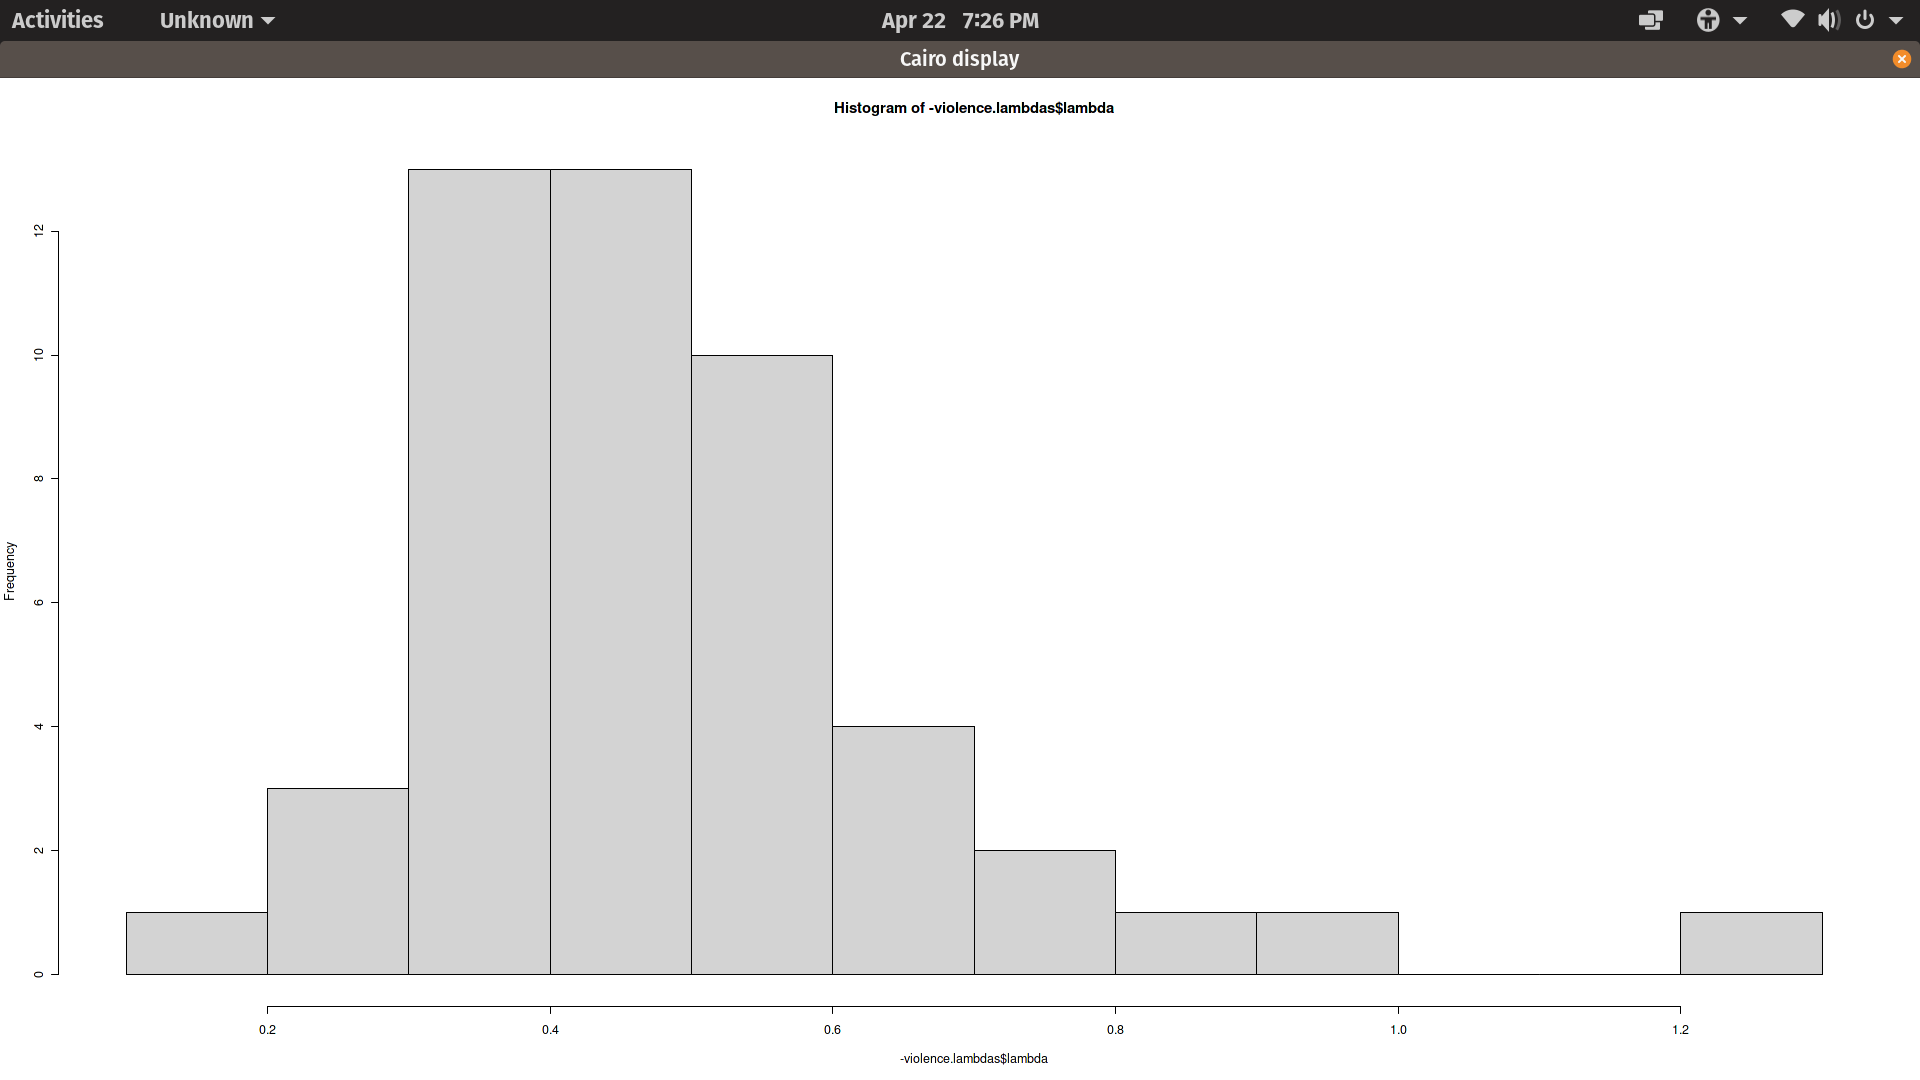
\includegraphics[scale=0.15]{hviol.png}

The mean is $\bar{\lambda}=0.49$ and $\sigma(\lambda) =0.18$.

The GHD fit is
\begin{verbatim}
> summary(fit.violence)
Warning: fitting procedure did not converge!

Asymmetric Generalized Hyperbolic Distribution:

Parameters:
    lambda  alpha.bar         mu      sigma      gamma 
-1.9111168  0.7435190  0.3898858  0.1493979  0.1002899 

Call:
fit.ghypuv(data = -violence.lambdas$lambda)

Optimization information:
log-Likelihood:                21.368 
AIC:                           -32.736 
Fitted parameters:             lambda, alpha.bar, mu, sigma, gamma;  (Number: 5)
Number of iterations:          502 
Converged:                     FALSE 
Error code:                    1 
Error message:       
\end{verbatim}

\section{Idea for Bounds on Murder Rate 2 Million Years Ago}

Being originally a mathematics student, I like to take a broad view about the {\em violent nature} of our pre-human ancestors.  Australopithecus africanus was roughly 4 million years ago and were bipedal.  Robert Ardrey's {\em African Genesis} depited a violent nature to our primate ancestors in Africa.  We have fossils of Homo Habilis from around 2 million years ago.  I want to have some sensible numbers for violence; for example murder rates.  Today around the world murder rates are bounded above roughly by 0.08 percent.  I would like some accurate bounds for the last 2 million years.  

To understand this point of view, if we set the murder rate 2 million years ago to 10\%, we might run into extinction of the species.  That is quite high.  On the other hand, it will be difficult to believe that the murder rate was below 0.001\% because that's better than what we have today, and violence has gone down in the last 2 million years. 
I don't have a good answer at all to murder rate over 2 million years but I think the question is important to resolve.  Our ideas about the true savagery of our primate ancestors need to be roughly accurate in order for us to make progress.


\end{document}